\clearpage\section{Vertical Stretches}
A close second in terms of simplicity is the vertical stretch, represented by the letter $a$. This function multiplies every output of a function by its value. For example, if $f(x) = x$, the function $g(x) = 2x$, where $a = 2$, means that every value plugged into $g(x)$ is doubled. Likewise, if we set $a = \dfrac{1}{2}$, every value plugged into a new function $h(x) = \dfrac{1}{2}x$ is halved.
\begin{center}
    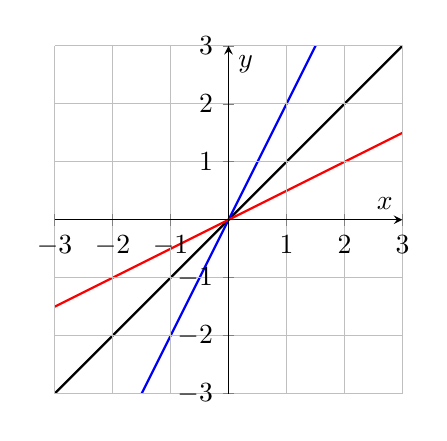
\begin{tikzpicture}
        \begin{axis} [
            axis lines=middle,
            xlabel = $x$, ylabel = {$y$},
            xmin = -3, xmax = 3,
            ymin = -3, ymax = 3,
            xtick distance={1}, ytick distance={1},
            grid = both,
            width = 6cm,
            height = 6cm,
            smooth,
            axis on top
        ]

            \addplot[black, thick, smooth, domain = -3:3, samples = 100]{x};
            \addplot[blue, thick, smooth, domain = -3:3, samples = 100]{2 * x};
            \addplot[red, thick, smooth, domain = -3:3, samples = 100]{(1 / 2) * x};
        \end{axis}
    \end{tikzpicture}\\
    $f(x) = x$ (Black), 
    $g(x) = 2x$ (Blue),
    $h(x) = \dfrac{1}{2}x$ (Red) \\
    \textit{Note that $a$ for a linear function is its slope.}
\end{center}

\begin{definition}
    Given a function $f(x)$ and a vertical stretch $a$, the new function $g(x) = af(x)$ is the function where every value in the range of $f$ is multiplied by $a$.
    \begin{itemize}
        \item When $a > 1$, stretching occurs.
        \item When $0 < a < 1$, compression occurs.
        \item When $a = 1$, the function is unaffected. 
        \item When $a = 0$, the function is a horizontal line.
    \end{itemize}
\end{definition}
